\section{Entwurf}
\subsection{Geschäftsfälle anhand des BPMN Workflows}
\subsection{Auswahl und Begründung des Datenbankkonzepts}
Die Lern-App \gqq{LearnAhead} benötigt eine Datenbank, um die Lerninhalte des Benutzers speichern zu können. Die Datenbank soll hierbei die folgenden Anforderungen erfüllen:
\begin{itemize}
    \item Es soll möglich sein, Bilder einfach zu speichern und abzurufen.
    \item Die Datenbank soll gut skalierbar sein, um auch bei vielen Benutzern eine gute Performance zu gewährleisten.
    \item Es müssen gute Frameworks zur Anbindung für die Sprache Kotlin existieren.
    \item Die Datenbank soll in der Cloud gehostet werden, um die Wartungskosten zu minimieren.
    \item Die Datenbank soll möglichst kostenlos sein.
\end{itemize}

\noindent
Hierbei gab es die Entscheidung zwischen einer relationalen und einer NoSQL Datenbank. Da diese für die Speicherung von Bildern zuständig ist, ist eine NoSQL Datenbank die bessere Wahl. In diesem Zusammenhang kam der Anbieter \gqq{Firebase} in Frage. Dieser bietet zwei unterschiedliche Datenbanken an: \gqq{Cloud Firestore} und \gqq{Realtime Database}. Realtime Database wird genutzt, wenn die Datenbank in Echtzeit synchronisiert werden soll. Da dies bei der Lern-App nicht notwendig ist, wurde sich für Cloud Firestore entschieden. Cloud Firestore baut auf den Erfolgen von Realtime Database auf und bietet zusätzlich eine bessere Skalierbarkeit und ermöglicht zudem schnellere Abfragen. \cite*{Firestore} Für die Speicherung von Inhalten gibt es den Firebase Storage, welcher eine einfache Möglichkeit bietet, Inhalte wie z.B. Bilder oder Videos zu speichern. \newline

\noindent
Firebase bietet eine gute Anbindung für Kotlin (siehe \ref*{Auswahl BibliothekenFrameworks}). Zusätzlich ist Firebase kostenlos, solange die Datenbank nicht zu groß wird. Hierbei kann eine monatliche Anzahl von 50.000 Nutzern, 20.000 Schreibvorgängen und 50.000 Lesevorgängen kostenlos genutzt werden. Der Speicherplatz für den Firebase Storage beträgt 1 GB, welcher für die Lern-App ausreichend ist. \cite*{Firebase_Pricing}
\subsection{Auswahl von wichtigen Bibliotheken/Frameworks} \label{Auswahl BibliothekenFrameworks}
In diesem Abschnitt werden die wichtigsten in LearnAhead verwendeten Bibliotheken und Frameworks erläutert. Es wird kurz darauf eingegangen was genau die/das Bibliothek/Framework tut und wieso sie über andere gewählt wurde.
\subsubsection{DaggerHilt Dependency Injection Framework}
DaggerHilt ist ein Framework für Dependency Injection (DI), das speziell für Android entwickelt wurde \cite{Dagger2021}. Es basiert auf Dagger, einem weit verbreiteten und mächtigen DI-Framework für Java \cite{AndroidDevelopers2021}. \newline
Dependency Injection ist ein Programmierparadigma, das dabei hilft, Objekte effizient zu erzeugen und zu verwalten. Mit Hilfe von DaggerHilt können Abhängigkeiten zentral verwaltet und bei Bedarf ausgetauscht werden. Das ermöglicht bessere Testbarkeit und modulareren Code, da jede Klasse sich nur auf ihre Aufgaben konzentrieren muss und ihre Abhängigkeiten von außen erhält \cite{Dagger2021}. \newline
Die Wahl von DaggerHilt für diese Arbeit beruht auf seiner tiefen Integration in das Android-Ökosystem. DaggerHilt ist in der Lage, Abhängigkeiten über die Grenzen von Aktivitäten, Fragmenten und Services hinweg zu verwalten und ist dabei eng mit dem Lebenszyklus von Android-Anwendungen verbunden \cite{AndroidDevelopers2021}. \newline
Darüber hinaus unterstützt DaggerHilt das Konzept der Compile-Time Injection. Das bedeutet, dass Abhängigkeiten zur Kompilierzeit aufgelöst werden, was die Fehlererkennung verbessert und Laufzeitfehler minimiert \cite{Dagger2021}. \newline
\subsubsection{Markwon: Eine Markdown-Bibliothek für Android}
Markwon ist eine leistungsfähige Bibliothek, die speziell entwickelt wurde, um die Anzeige und Formatierung von Markdown-Inhalten auf Android zu erleichtern \cite{Markwon2022}. Markdown ist eine leichtgewichtige und benutzerfreundliche Markup-Sprache, die oft für die Formatierung von Text in Softwareentwicklungsprojekten, Dokumentationen und im Web verwendet wird \cite{Gruber2004}. \newline
Bei LearnAhead wird der Input mit einem in Markwon enthaltenen Editor eingegeben und daraufhin in einem Android freundlichen Format in einem TextView angezeigt. \newline
Die Markwon-Bibliothek bietet eine voll funktionsfähige Markdown-Rendering-Engine für Android, die in einer TextView-Komponente arbeitet. Sie unterstützt alle gängigen Markdown-Syntaxelemente und bietet zusätzlich Funktionen wie Syntaxhervorhebung für Codeblöcke, Inline-Latex-Rendering und vieles mehr \cite{Markwon2022}. \newline
Für diese Arbeit wurde Markwon aufgrund seiner hohen Flexibilität und seiner vielfältigen Funktionen gewählt. Durch die Nutzung der Markwon-Bibliothek können komplexe, formatierte Textinhalte in der Android-Anwendung auf einfache und effiziente Weise angezeigt werden \cite{Markwon2022}. \newline
\subsubsection{Glide: Ein Framework zum Laden von Bildern in Android}
Glide ist ein effizientes Open-Source-Framework zur Handhabung und Darstellung von Bildern und Videos in Android-Anwendungen \cite{Glide2022}. Es wurde von Bumptech entwickelt und ist bekannt für seine Leistung, insbesondere bei der Scroll-Leistung in Listen oder Rastern von Bildern. \newline
In LearnAhead wird Glide beispielsweise dafür genutzt, um die Profilbilder der Nutzer zu laden. Eine der Hauptfunktionen von Glide ist das asynchrone Laden und Speichern von Bildern aus verschiedenen Quellen, beispielsweise aus dem Internet, ohne den Haupt-UI-Thread zu blockieren. Dies führt zu einer glatteren Benutzererfahrung \cite{Glide2022}. Zudem bietet Glide auch Funktionen wie das Zuschneiden und Transformieren von Bildern, das Cachen von Bildern für eine schnellere Wiederverwendung und die automatische Verwaltung des Lebenszyklus \cite{GlideGithub2022}. \newline
Die Wahl von Glide für diese Arbeit basiert auf seinen umfangreichen Funktionen, seiner Leistung und seiner Integration in das Android-Ökosystem. Mit Glide können komplexe Bildverarbeitungsanforderungen erfüllt werden, während gleichzeitig die Performance und die Benutzererfahrung der App optimiert werden \cite{Glide2022}. \newline
\subsubsection{Android Navigation: Ein Framework zur Navigation in Android-Anwendungen}
Android Navigation ist eine Bibliothek, die von Google entwickelt wurde und das Navigieren zwischen den verschiedenen Bildschirmen einer Android-Anwendung erleichtert \cite{AndroidNav2022}. Es ist Teil der Android Jetpack-Bibliotheken, einer Sammlung von Bibliotheken, Tools und Leitlinien, die robuste und wartungsfreundliche Android-Apps unterstützen \cite{AndroidJetpack2022}. \newline
In LearnAhead wird die Bibliothek für die Navigation zwischen den verschiedenen Fragments (Teil-Bildschirmen) der App genutzt. Mit dem Android Navigation Framework können Entwickler visuell oder programmgesteuert einen Navigationspfad zwischen den verschiedenen Komponenten einer App erstellen, z. B. zwischen verschiedenen Aktivitäten oder Fragmenten. Die Bibliothek sorgt dafür, dass die Benutzeroberfläche in einem konsistenten und vorhersehbaren Zustand bleibt und beinhaltet auch Unterstützung für erweiterte Navigationsszenarien wie tiefe Links und Navigationsleisten \cite{AndroidNav2022}. \newline
Die Wahl dieses Frameworks für diese Arbeit beruht auf seiner Integration in das Android-Ökosystem und seinen umfangreichen Funktionen zur Handhabung von App-Navigationsszenarien. Die Verwendung des Android Navigation Frameworks erleichtert die Erstellung von strukturierten und benutzerfreundlichen Navigationsflüssen in der App \cite{AndroidNav2022}. \newline
\subsubsection{Firebase Android SDK: Eine Bibliothek zur Integration von Firebase in Android-Anwendungen}
Firebase Android SDK ist eine Bibliothek, die eine Anbindung an Firebase und dessen verschiedenen Dienste ermöglicht \cite{FirebaseSDK2022}. Firebase, entwickelt von Google, ist eine Plattform, die verschiedene Backend-Services wie Datenbanken, Authentifizierung, Cloud-Funktionen, Hosting und mehr bietet \cite{Firebase2022}. \newline
In LearnAhead wird die Bibliothek genutzt, um die Verbindung zur Firebase-Datenbank herzustellen. Die Firebase Android SDK bietet Funktionen zur nahtlosen Integration dieser Dienste in Android-Anwendungen. Es bietet eine Reihe von APIs und Konfigurationstools, die es Entwicklern ermöglichen, auf leistungsfähige Weise auf Firebase-Dienste zuzugreifen und diese in ihren Apps zu nutzen \cite{FirebaseSDK2022}. \newline
Die Entscheidung, Firebase Android SDK für diese Arbeit zu nutzen, basiert auf seiner umfangreichen Integration in das Firebase-Ökosystem und seiner Fähigkeit, robuste und skalierbare Backend-Services bereitzustellen. Die Verwendung von Firebase Android SDK erleichtert den Zugriff auf und die Verwaltung von Firebase-Diensten innerhalb der Android-Anwendung \cite{FirebaseSDK2022}. \newline

\subsection{Wahl des Architektur-Patterns: Model-View-ViewModel (MVVM)} \label{Wahl des Architektur-Pattern}
Bei der Entwicklung von Software ist die Wahl des richtigen Architektur-Patterns von entscheidender Bedeutung. Für diese Arbeit wurde das Model-View-ViewModel (MVVM) Pattern gewählt, welches sich in den letzten Jahren zu einem der Standard-Architektur-Patterns für Android-Entwicklung etabliert hat \cite{AndroidAppArchitecture}. \newline
MVVM teilt die Anwendungslogik in drei miteinander verbundene Komponenten auf: das Model, die View und das ViewModel \cite{MicrosoftMVVM2022}. Das Model repräsentiert die Daten und die Geschäftslogik der Anwendung. Die View ist verantwortlich für die Darstellung der Daten und die Interaktion mit dem Benutzer. Das ViewModel fungiert als Bindeglied zwischen Model und View und stellt die Daten für die View zur Verfügung und reagiert auf Benutzeraktionen \cite{AndroidAppArchitecture}. \newline
MVVM hat mehrere Vorteile, darunter eine klare Trennung von Anliegen, verbesserte Testbarkeit und eine bessere Unterstützung für reaktive Programmierung \cite{AndroidAppArchitecture}. Diese klare Trennung der Anliegen ermöglicht es, dass verschiedene Teile der Anwendung unabhängig voneinander entwickelt und getestet werden können, was zu einer besseren Code-Qualität und Wartbarkeit führt \cite{MicrosoftMVVM2022}. \newline
\begin{figure}[h]
    \centering
    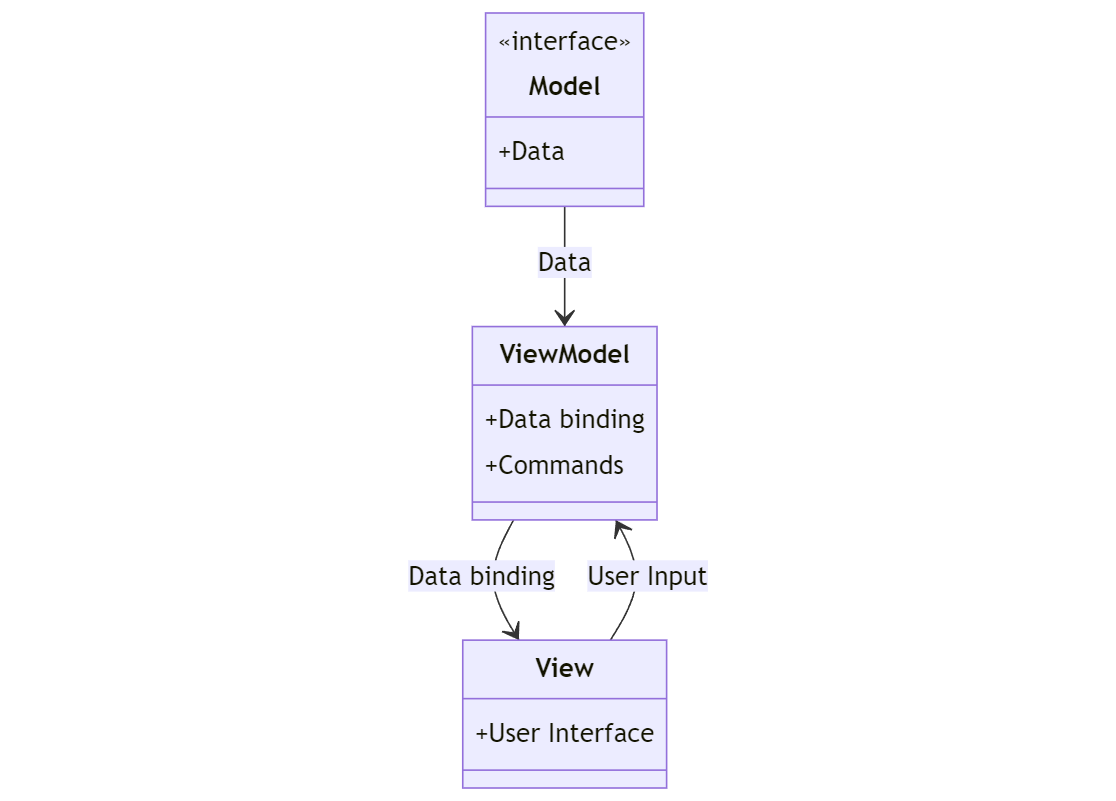
\includegraphics[width=0.75\textwidth]{images/diagramme/MVVM.png}
    \caption{MVVM Diagramm}
    \label{fig:mvvm}
\end{figure}
    
Das in Abbildung \ref{fig:mvvm} dargestellte Diagramm zeigt das Model-View-ViewModel (MVVM) Designmuster. Dieses Muster wird häufig in der Softwareentwicklung verwendet, insbesondere in Anwendungen mit grafischer Benutzeroberfläche. Es besteht aus drei Hauptkomponenten:

\begin{itemize}
\item \textbf{Model}: Dies repräsentiert die Daten und die Geschäftslogik der Anwendung. Es ist unabhängig von der Benutzeroberfläche und enthält keine Informationen darüber, wie die Daten dargestellt werden.
\item \textbf{View}: Dies ist die Benutzeroberfläche der Anwendung. Sie zeigt die Daten an, die vom Model bereitgestellt werden, und sendet Benutzereingaben an das ViewModel.
\item \textbf{ViewModel}: Dies ist das Bindeglied zwischen Model und View. Es holt Daten vom Model, führt eventuell notwendige Transformationen durch und stellt sie der View zur Verfügung. Außerdem verarbeitet es Benutzereingaben von der View und führt entsprechende Aktionen im Model aus.
\end{itemize}
\subsection{Software-Komponenten}
Das System wird zunächst als Gesamtkomposition dargestellt. Anschließend werden die Subsysteme einzeln dargestellt. 
\subsubsection{Gesamtkomposition}
\begin{figure}[H]
    \centering
    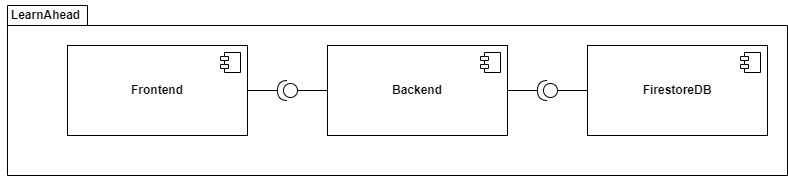
\includegraphics[width=0.8\textwidth]{images/diagramme/Gesamtkomposition.png}
    \caption{Gesamtkomposition}
    \label{fig:Gesamtkomposition}
\end{figure}
\noindent
Die Gesamtkomposition besteht aus den folgenden Subsystemen:
\begin{itemize}
    \item \textbf{Frontend:} Das Frontend ist für die Darstellung der Benutzeroberfläche zuständig. Es kommuniziert mit dem Backend, um Daten anzuzeigen und Eingaben an dieses weiterzuleiten.
    \item \textbf{Backend:} Das Backend ist für die Verarbeitung und Validierung der Daten zuständig. Es kommuniziert mit der FireStore Datenbank, um Daten abzurufen und zu speichern.
    \item \textbf{FireStoreDB} Die FireStoreDB Komponente ist die Datenbank-Komponente.
\end{itemize}

\noindent
Näheres hierzu im Deployment Diagramm \ref*{Deployment Diagramm} und Klassen Diagramm \ref*{Klassen Diagramm}.
\newpage
\subsubsection{Frontend}
Es gibt zwei Diagramme für das Frontend. Das Diagramm \ref*{fig:FrontendUINavigation} zeigt die Navigation zwischen den einzelnen Pages.
\begin{figure}[H]
    \centering
    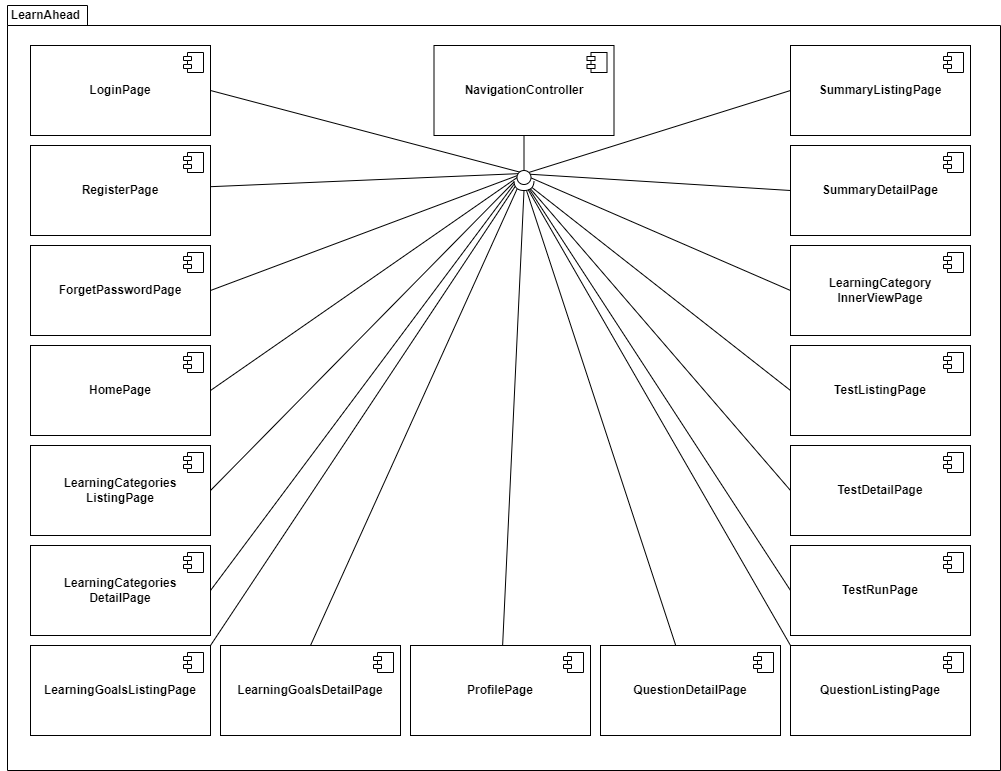
\includegraphics[width=0.8\textwidth]{images/diagramme/FrontEndKomposition.png}
    \caption{Frontend UI Navigation}
    \label{fig:FrontendUINavigation}
\end{figure}
\noindent
Das Diagramm \ref*{fig:FrontendUIViewModel} zeigt die Kommunikation zwischen den einzelnen Pages und dem ViewModel. Hierbei ist zu beachten, dass dieses Diagramm die Kommunikation zwischen den einzelnen Pages und dem ViewModel im Allgemeinen zeigt. Das bedeutet, dass jede Page ein zugehöriges ViewModel hat. Die Kommunikation zwischen den einzelnen Pages und dem ViewModel ist prinzipiell immer gleich. Weitere Details sind in Kapitel \ref*{Wahl des Architektur-Pattern} zu finden. \newline
\begin{figure}[H]
    \centering
    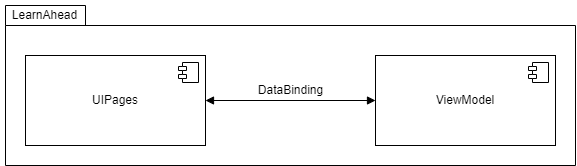
\includegraphics[width=0.8\textwidth]{images/diagramme/UIPagesMitViewModel.png}
    \caption{Frontend UI Kommunikation mit ViewModel}
    \label{fig:FrontendUIViewModel}
\end{figure}
\subsubsection{Backend}
Das Diagramm \ref*{fig:BackendKomposition} zeigt die Komposition des Backends. Hierbei ist zu beachten, dass dieses Diagramm die Komposition des Backends im Allgemeinen zeigt. Jedes Objekt, welches in der Datenbank gespeichert wird, hat ein zugehöriges Repository/Model. Die Kommunikation zwischen den verschiedenen Repositories und Modellen verläuft grundsätzlich immer auf die gleiche Weise. Jedes Repository baut auf einem Interface auf, welches die grundlegenden Funktionen für die Kommunikation mit der Datenbank definiert. Die Kommunikation mit der Datenbank erfolgt über das Repository.
\begin{figure}[H]
    \centering
    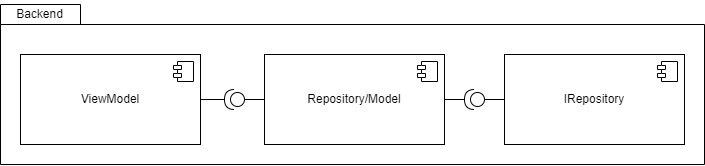
\includegraphics[width=0.8\textwidth]{images/diagramme/Backend.png}
    \caption{Backend Komposition}
    \label{fig:BackendKomposition}
\end{figure}
\subsection{Deployment Diagramm} \label{Deployment Diagramm}
\subsection{Klassen Diagramm} \label{Klassen Diagramm}
\subsection{Aktivitätsdiagramm}
\subsection{Sequenzdiagramme}
\subsection{Prototyp (optional)}